
\chapter{Mise en \oe{}uvre de \PpFf}
\label{implementation.chap}


Ce chapitre pr\'esente une description d\'etaill\'ee de la fa\c{c}on dont \TT{PpFf} est impl\'ement\'e. 
%
De fa\c{c}on g\'en\'erale, la mise en \oe{}uvre est bas\'ee sur la biblioth\`eque \TT{FastFlow}, h\'eritant et \'etendant plusieurs de ses classes. La premi\`ere section d\'ecrit bri\`evement les diff\'erents éléments composant la biblioth\`eque \TT{PpFf}. La deuxi\`eme section montre les couches de \TT{PpFf} et les liens entre elles. La troisi\`eme section d\'ecrit comment le pipeline du flux est mis en œuvre. La section suivante examine comment la parall\'elisation du flux est r\'ealis\'ee. Les \emph{stages} sont d\'ecrits dans la cinqui\`eme section. La dernière section pr\'esente la description d'un exemple complet d\'ecrivant comment un programme \PpFf{} est compil\'e et ex\'ecut\'e. Afin de donner un aper\c{c}u de l'envergure du projet r\'ealis\'e, quelques donn\'ees sur le code de cette mise en \oe{}uvre sont pr\'esentées dans l'annexe~\ref{QuelquesDonneesSurLaMiseEnOeuvre.ann}.


\section{Les principaux éléments de \TT{PpFf}}

\begin{figure}
\centering
     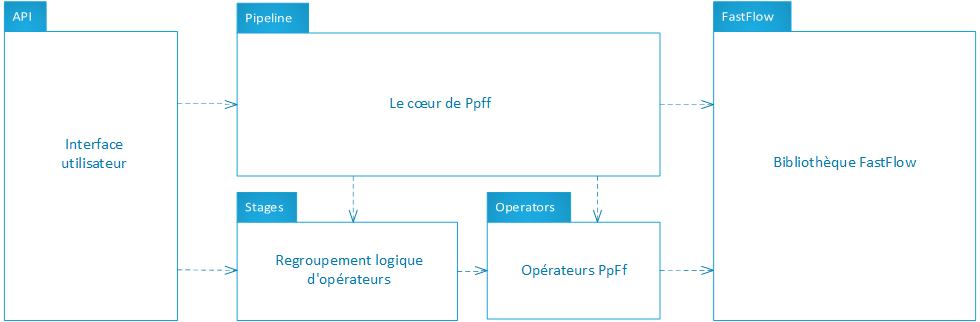
\includegraphics[width=1.0\textwidth]{Figures/ComponentsPpFf.png}
      \caption{Les principaux éléments de \TT{PpFf}.}
       \label{AllComponentsAPI.fig}
\end{figure}

\TT{PpFf} est impl\'ement\'e en utilisant plusieurs éléments, c'est-à-dire, plusieurs classes. Une vue d'ensemble de ces éléments est illustrée dans la figure~\ref{AllComponentsAPI.fig}. 

\begin{itemize}

\item Le point d'entrée de \ppff\ est la classe \TT{Flow}, avec laquelle interagissent les d\'eveloppeurs pour créer des flux de traitement. Toutes les op\'erations de traitement d'un flux de \TT{PpFf} sont li\'ees aux m\'ethodes expos\'ees par cette classe. 

\item Le c\oe{}ur du traitement de \TT{PpFf} est le \TT{Pipeline}. La cr\'eation et l'ex\'ecution d'un flux sont g\'er\'ees par celui-l\`a. 

\item Dans l'éléments \TT{Operators}, on retrouve tous les op\'erateurs d\'efinis dans \TT{PpFf}%
%
\GT{qui font... quoi? Il faudrait décrire brièvement (1 phrase) à quoi servent ces opérateurs}
.
%
Ces op\'erateurs sont expos\'es \`a l'utilisateur par le biais de l'\TT{API} de \TT{PpFf}. 

\item L'élément \TT{Stages} permet de regrouper un ou plusieurs op\'erateurs en un seul objet composite. On verra à la section~\ref{stages.sect} qu'il est utilisé lorsqu'on crée, avec \TT{parallel()}, une instance d'un \TT{farm} parallèle avec plusieurs travailleurs. 

\item Le dernier élément, \TT{FastFlow}, est la biblioth\`eque au–dessus de laquelle \TT{PpFf} est impl\'ement\'e.


\end{itemize}

\section{Mise en \oe{}uvre multi-couches de \PpFf{} via \TT{FastFlow}}

\begin{figure}
\centering
     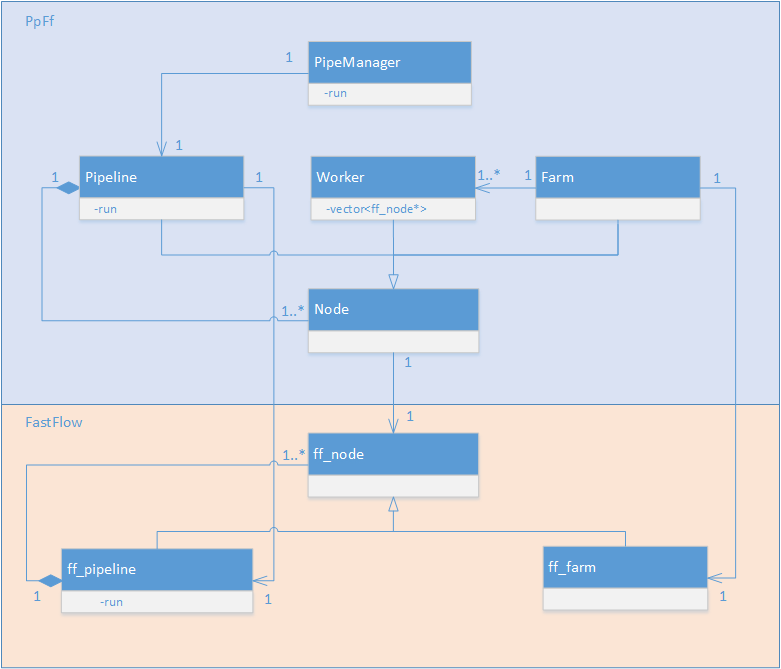
\includegraphics[width=1.0\textwidth]{Figures/CorrespondencePpFfToFastFlow.png}
      \caption{La correspondance entre les \'el\'ements de \TT{PpFf} et ceux de  \TT{FastFlow}.}
       \label{CorrespondencePpFfToFastFlow.fig}
\end{figure}

\TT{PpFf} est impl\'ement\'e au–dessus de la biblioth\`eque \TT{FastFlow}, de sorte que nous utilisons les constructions \TT{ff\_node}, \TT{ff\_pipeline} et \TT{ff\_farm} de \TT{FastFlow}. La figure~\ref{CorrespondencePpFfToFastFlow.fig} montre la correspondance entre les \'el\'ements de \TT{PpFf} et ceux de \TT{FastFlow}. 


\GT{Ci-bas: J'ai modifié car ce n'était pas clair ce que signifiait
<<Ces classes de correspondance>>. À vérifier si c'est ok!?}

Les classes \TT{PipeManager}, \TT{Pipeline}, \TT{Node} et \TT{Farm} sont les classes principales de \TT{Pipeline}, le c\oe{}ur du traitement de \TT{PpFf}. Alors que la classe \TT{PipeManager} g\`ere la cr\'eation et l'ex\'ecution d'une instance d'un pipeline, la classe \TT{Pipeline} g\`ere la cr\'eation du flux de traitement associé. Un flux de traitement, dans \TT{PpFf}, est compos\'e d'un ou plusieurs \emph{op\'erateurs}, lesquels h\'eritent de la classe \TT{Node}. Un \TT{Node} peut \^etre un \TT{Pipeline}, un \TT{Worker} ou un \TT{Farm}. Les classes \TT{Worker} et \TT{Farm} sont utilis\'ees pour cr\'eer les instances parall\`eles d'un \TT{farm} --- voir plus bas.

Chaque classe principale susmentionn\'ee de \TT{FastFlow} a une classe correpondante dans \TT{PpFf}. Par exemple, l'impl\'ementation de la classe \TT{Node} de \TT{PpFf} est r\'ealis\'ee par l'entremise de la classe \TT{ff\_node} de \TT{FastFlow}. Ce m\'ecanisme a permis d'ajouter plus de fonctionnalit\'es \`a l'API tout en b\'en\'eficiant des fonctionnalités et performances offertes par \TT{FastFlow}.



\section{Mise en \oe{}uvre des pipelines}

Un pipeline, un objet de classe \TT{Pipeline}, repr\'esente une cha\^ine de traitement. Un \TT{Pipeline} est compos\'e par une s\'erie d'op\'erations sp\'ecifi\'ees par l'utilisateur qui sont appliqu\'ees aux \'el\'ements d'un flux. Comme on peut le voir dans la figure~\ref{CorrespondencePpFfToFastFlow.fig}, un \TT{Pipeline} utilise les fonctionnalit\'es de la classe \TT{ff\_pipeline} de \TT{FastFlow}. 

Celles qui composent un \TT{Pipeline} sont de deux types : les op\'erations sans \'etat et avec \'etat. Un \TT{Pipeline} contient une ou plusieurs op\'erations sans \'etat et une seule op\'eration avec \'etat. Lorsque cette derni\`ere est ajout\'ee dans le \TT{Pipeline}, la m\'ethode \TT{run()} du \TT{Pipeline} est appel\'ee. \`A ce stade, un objet de type \TT{ff\_pipeline} correspondant au \TT{Pipeline} est cr\'e\'e. Ensuite, chaque op\'eration sp\'ecifi\'ee par l'utilisateur est visit\'ee et, en fonction de la configuration \'etablie, des objets de type \TT{ff\_node} ou \TT{ff\_farm} sont ajout\'es dans l'objet \TT{ff\_pipeline}. Chaque nœud ainsi ajout\'e dans \TT{ff\_pipeline} sera alors ex\'ecut\'e dans un fil d'ex\'ecution ind\'ependant (\emph{thread}), une caract\'eristique de la mise en \oe{}uvre de \TT{FastFlow}.
%La cr\'eation d'un \TT{Pipeline} est r\'ealis\'ee \`a l'aide de la classe \TT{PipeManager}, dont les d\'etails sont omis.


\section{\'Ex\'ecution parall\`ele avec parall\'elisme de flux ou de donn\'ees}

La cr\'eation de code parall\`ele est g\'en\'eralement consid\'er\'ee du domaine d'experts. La complexit\'e de l'\'ecriture de code parall\`ele diminue la productivit\'e, ce qui peut augmenter les co\^uts de d\'eveloppement. Par contre, \TT{PpFf} permet aux programmeurs de composer des morceaux de code s\'equentiel --- des fonctions ou expressions lambdas --- et d'ex\'ecuter le tout en parall\`ele.
%
L'objectif de cette section est de d\'ecrire les deux types de parall\'elisme impl\'ement\'es dans \TT{PpFf}, utilisables 
%
par l'interm\'ediaire d'une unique interface : le parall\'elisme de flux et le parall\'elisme de donn\'ees.



\subsection{Parall\'elisme de flux}

Le parall\'elisme de flux consiste \`a ex\'ecuter plusieurs \'etapes d'un traitement s\'equentiel en parall\`ele en leur faisant traiter des donn\'ees diff\'erentes. Les donn\'ees se succ\`edent ainsi les unes aux autres dans les diff\'erentes \'etapes --- appel\'ees  aussi des \emph{stages} (cf.~Section~\ref{stages.sect}).
%
Dans \TT{PpFf}, un \emph{stage} est cr\'e\'e et ajouté au pipeline de traitement dès lors qu'une m\'ethode de l'interface de \TT{PpFf} est ajout\'ee au \emph{pipeline}, par l'intermédiaire du cha\^inage de m\'ethodes.
%
Le traitement effectu\'e dans un \emph{stage} \`a un instant donn\'e peut d\'ependre, ou non, des traitements effectu\'es par ce m\^eme \emph{stage} pour les donn\'ees pr\'ec\'edentes --- un \'etat interne peut donc \^etre conserv\'e. 
%
\`A noter que ce type de parall\'elisme est appliqu\'e par d\'efaut dans notre biblioth\`eque. 
%
Ce fonctionnement permet de parall\'eliser des traitements avec des d\'ependances entre les donn\'ees sans avoir recours \`a des synchronisations \emph{explicites} par le programmeur. 

\goodbreak
\begin{samepage}
Un flux compos\'e de $n$ \emph{stages} $S_1, S_2, \ldots, S_n$ o\`u le \emph{stage} $S_i$ ex\'ecute une op\'eration $O_i$ peut \^etre exprim\'e sous la forme d'une composition s\'equentielle d'op\'erations sur les \'el\'ements d'entr\'ee comme suit, o\`u $O(x)$ repr\'esente le traitement global d'un \'el\'ement $x$ du flux~: 
%
\[
	O(x) = O_n( \ldots (O_k( \ldots O_1(x)) \ldots ) \ldots ));
\]
\end{samepage}


\begin{figure}
\centering
     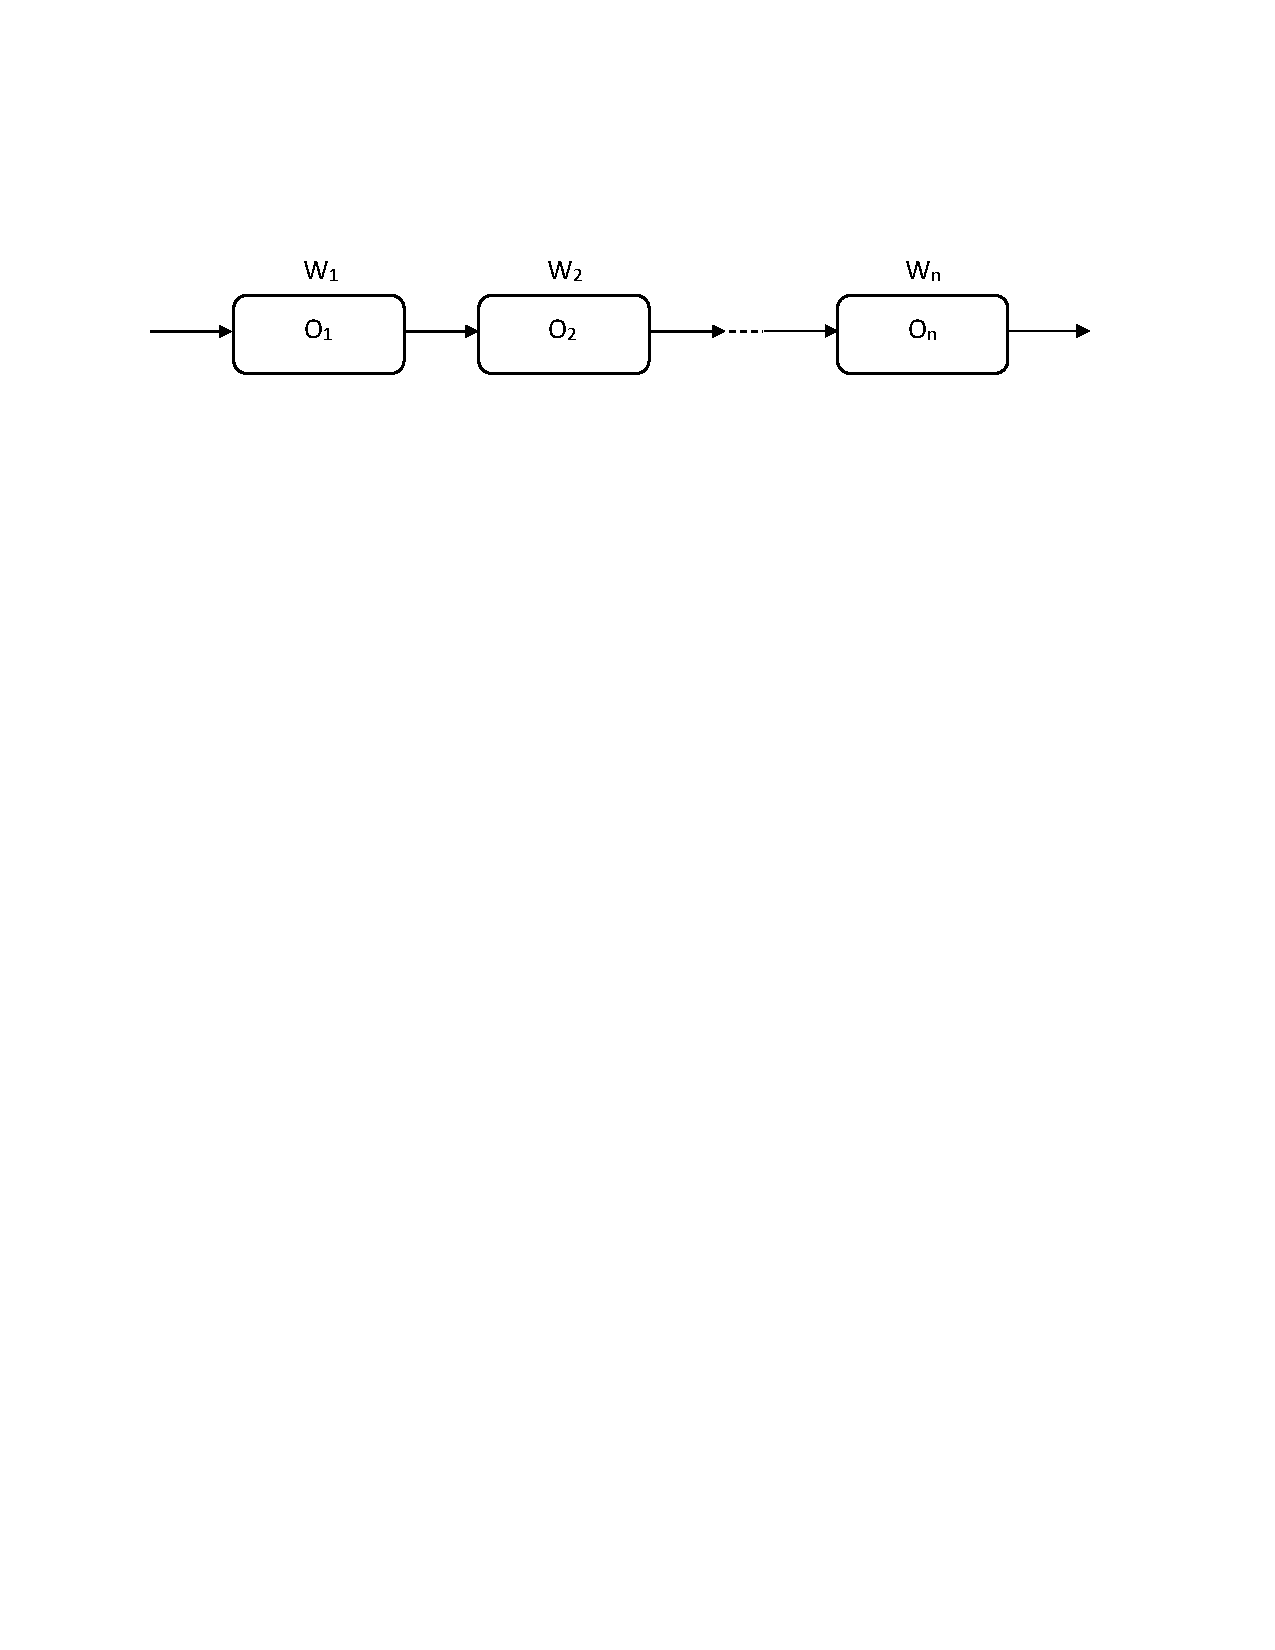
\includegraphics[width=1.0\textwidth]{Figures/ParallelismeDuFlux.pdf}
      \caption[Une repr\'esentation graphique du parall\'elisme de flux en \ppff.]{Une repr\'esentation graphique du parall\'elisme de flux pour une d\'ecomposition en $n$ \emph{stages} $S_1, S_2, \ldots, S_n$. Les op\'erations $O_1, O_2, \ldots, O_n$ sont ex\'ecut\'ees de fa\c{c}on parall\`ele dans diff\'erents fils d'ex\'ecution $W_1, W_2, \ldots, W_n$ ($W$ pour \emph{$W$orker}).}
       \label{ParallelismeDuFlux.fig}
\end{figure}


Si on note par $W_i$ le fil d'ex\'ecution (\emph{thread}) associ\'e au \emph{stage} $S_i$, alors
le parall\'elisme de flux du pipeline peut \^etre repr\'esent\'e par un graphe lin\'eaire de $n$ travailleurs. Chaque travailleur correspond \`a une op\'eration sp\'ecifique $O_i$. La figure~\ref{ParallelismeDuFlux.fig} montre la repr\'esentation graphique du parall\'elisme de flux dans un tel pipeline. Signalons que cette solution n'acc\'el\`ere pas le calcul d'un seul \'el\'ement; par contre, elle am\'eliore \emph{le d\'ebit de sortie}.

\subsection{Parall\'elisme de donn\'ees}
\label{StagesDataParallel.sect}

Le parall\'elisme de donn\'ees impl\'ement\'e dans \TT{PpFf}  consiste \`a r\'epliquer une op\'eration sur un ensemble de travailleurs identiques. Autrement dit, il vise \`a effectuer un traitement identique sur un ensemble de donn\'ees ind\'ependantes les unes des autres. 
%
Dans notre impl\'ementation de \PpFf, le parall\'elisme de donn\'ees est mis en \oe{}uvre avec les \emph{Task Farm} de \TT{FastFlow}.


D\'ecrit \`a la section~\ref{farm.sect}, un \emph{Task Farm} est compos\'ee de trois entit\'es : un \emph{Emitter}, plusieurs instances de travailleurs (\emph{workers}) et un \emph{Collector}. Par d\'efaut, dans \PpFf{}, les \'el\'ements sont r\'epartis par un \emph{Emitter} aux divers travailleurs selon une politique \emph{round robin}.%
%
\footnote{Politique \emph{round robin}~: approche d'ordonnancement pour r\'epartir la charge du travail entre des \emph{threads}, avec une file d'attente circulaire. Cf.~\url{https://fr.wikipedia.org/wiki/Round-robin_(informatique)}.} 
%
Les travailleurs re\c{c}oivent les \'el\'ements d'entr\'ee et appliquent sur chacun l'op\'eration sp\'ecifi\'ee au pr\'ealable par l'utilisateur. Les r\'esultats sont ensuite envoy\'es vers le \emph{Collector} charg\'e de les collecter --- i.e., de les combiner --- puis de les transmettre sur le flux de sortie.

Dans \TT{FastFlow} un \emph{Task Farm} est cr\'e\'e en instanciant la classe \TT{ff\_farm}. Cette classe correspond \`a la classe \TT{Farm} de \TT{PpFf}. La figure~\ref{CorrespondencePpFfToFastFlow.fig} illustre cette relation\'ependance. Lorsqu'une instance de \TT{Farm} est ajout\'ee au \emph{pipeline}, le flux est divis\'e en sous-flux --- appel\'es les instances parall\`eles d'un \TT{farm}. Ceci est possible en utilisant la m\'ethode \TT{parallel} de l'API de \TT{PpFf}. Le nombre de sous-flux ainsi cr\'e\'es d\'epend de la valeur sp\'ecifi\'ee en param\`etre pour cette m\'ethode.  

Dans \TT{PpFf}, les \'el\'ements du flux sont trait\'es dans l'ordre d'arriv\'ee selon le principe \emph{FIFO}. La collection de plusieurs r\'esultats \`a l'aide de cette approche r\'esulte dans un flux sans ordre sur ses \'el\'ements. En effet, le \emph{Collector} transmet les \'el\'ements au flux de sortie dans l'ordre d'arriv\'ee. \'Etant donn\'e que plusieurs flux ind\'ependants sont impliqu\'es, cet ordre ne peut pas \^etre pr\'ed\'etermin\'e. Si le respect d'un  ordre sp\'ecifique est requis, l'utilisateur de l'API peut ajouter une op\'eration qui produit cet ordre. Par exemple, la m\'ethode \TT{sort} de l'API (cf.~annexe~\ref{methodes-api.ann}), effectue le tri des \'el\'ements du flux selon l'ordre sp\'ecifi\'e par la fonction \TT{compare} envoy\'e en param\`etre.

\begin{figure}
\centering
     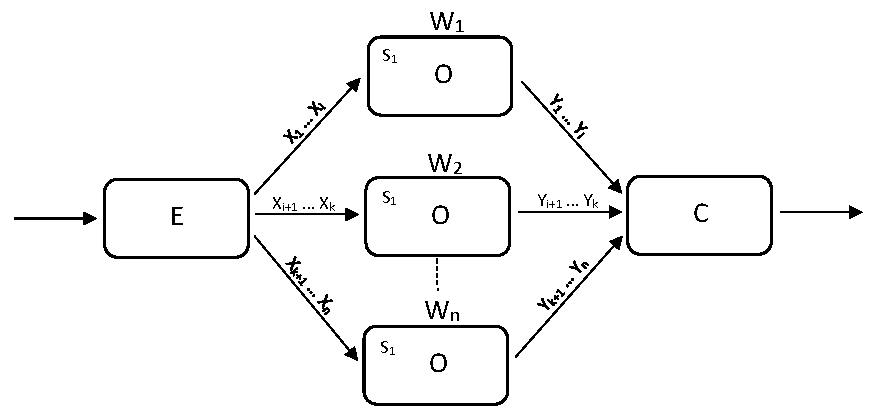
\includegraphics[width=1.0\textwidth]{Figures/DataParallelisme.pdf}
      \caption[Une repr\'esentation graphique du parall\'elisme de donn\'ees en \ppff.]{Une repr\'esentation graphique du parall\'elisme de donn\'ees. La m\^eme op\'eration~$O$ est ex\'ecut\'ee par les travailleurs $W_1, W_2,\ldots, W_n$ ($W$ pour \emph{$W$orker}). Le traitement associ\'e est repr\'esent\'e par le \emph{stage} $S_i$. Les \'el\'ements de donn\'ees sont r\'epartis entre les travailleurs par l'\'emetteur $E$ ($E$\emph{mitter}) puis les divers r\'esultats sont combin\'es par le collecteur $C$ ($C$\emph{ollector}).}
       \label{DataParallelisme.fig}
\end{figure}


L'impl\'ementation parall\`ele de ce mod\`ele peut \^etre
exprim\'ee sous la forme d'un ensemble de $n$ travailleurs $W_1, W_2,\ldots, W_n$ qui
appliquent une op\'eration $O$ sur les divers \'el\'ements~$X = \{x_1, \ldots, x_k\}$ apparaissant dans
le flux d'entr\'ee pour produire en sortie un ensemble d'\'el\'ements~$Y = \{y_1, \ldots, y_k\}$, o\`u $y_i = O(x_i)$.
%
Les divers \'el\'ements $x_i~(i=1, \ldots, k)$ sont r\'epartis entre
les travailleurs $W_j~(j=1, \ldots, n)$ d'une fa\c{c}on
ind\'etermin\'ee, qui d\'epend notamment de la vitesse de traitement
de chaque $x_i$.
%

La figure~\ref{DataParallelisme.fig} montre une repr\'esentation graphique du parall\'elisme de donn\'ees, o\`u la m\^eme op\'eration est ex\'ecut\'ee par les travailleurs $W_1, W_2,\ldots, W_n$. 

Il est possible de sp\'ecifier en param\`etre le nombre de travailleurs \`a utiliser pour l'ex\'ecution parall\`ele. Si ce param\`etre n'est pas sp\'ecifi\'e, un seul travailleur est activ\'e. Permettre ainsi d'augmenter le nombre de travailleurs fait en sorte qu'on peut augmenter le d\'ebit du traitement des donn\'ees si appropri\'e, c'est-\`a-dire, augmenter le nombre de donn\'ees qui peuvent \^etre trait\'ees en un temps donn\'e si le nombre de c\oe{}urs ou processeurs le permet.




\section{Stages}
\label{stages.sect}

\begin{figure}
\centering
     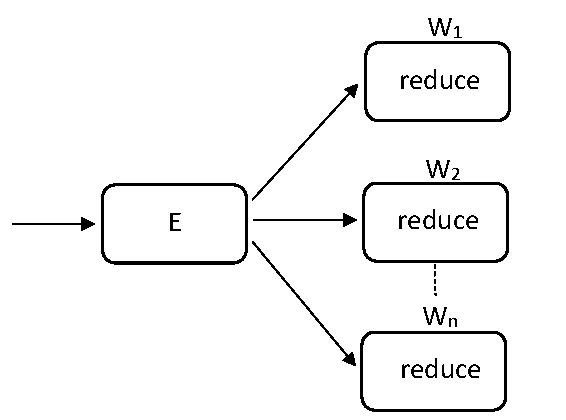
\includegraphics[width=0.7\textwidth]{Figures/StageDataParallel.pdf}
      \caption[Un exemple d'application de l'op\'eration \TT{reduce} sur diff\'erents sous-flux de donn\'ees.]{Un exemple d'application de l'op\'eration \TT{reduce} sur diff\'erents sous-flux de donn\'ees. C'est l'\emph{emitter} \TT{E} qui distribue les \'el\'ements $x_1, \ldots, x_k$ aux diff\'erents fils d'ex\'ecution $W_1, W_2, \ldots, W_n$ pour ainsi former les divers sous-flux de donn\'ees.}
       \label{StageDataParallel.fig}
\end{figure}



Le traitement en parall\`ele d'un flux de donn\'ees contribue \`a augmenter les performances du pipeline en utilisant les diff\'erents cœurs ou processeurs de la machine. Cependant, il existe une limitation lorsque le parall\'elisme est appliqu\'e en utilisant les instances parall\`eles d'un \emph{farm}. On rappelle qu'un flux est divis\'e en sous-flux lorsqu'un \emph{farm} est ajout\'e au \emph{pipeline}. Les r\'esultats partiels obtenus par les divers sous-flux de donn\'ees ainsi cr\'e\'es doivent \^etre combin\'es pour obtenir le r\'esultat global du traitement du flux. 

Par exemple, la figure~\ref{StageDataParallel.fig} montre un exemple o\`u une op\'eration \TT{reduce} est appliqu\'ee en parall\`ele sur un flux d'\'el\'ements $x_1, \ldots, x_k$. Or, le r\'esultat global correct doit \^etre obtenu \emph{en combinant les r\'esultats du traitement de chacun des sous-flux} trait\'es dans chaque fil d'ex\'ecution ind\'ependant. Afin de permettre un tel traitement, nous avons introduit les \emph{stages}. 


\begin{figure}
\centering
     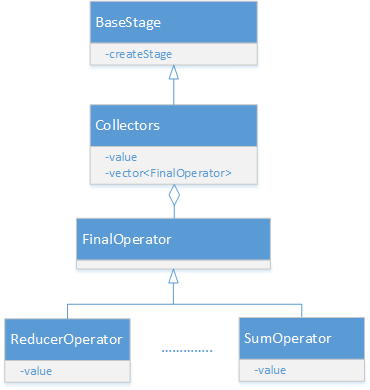
\includegraphics[width=0.7\textwidth]{Figures/StagesClassDiagramme.png}
      \caption{Le diagramme de classes pour la classe \texttt{Stage} et les classes associ\'ees.}
       \label{StagesClassDiagramme.fig}
\end{figure}


Un \emph{stage} repr\'esente le groupement logique d'une ou plusieurs op\'erations d'une \'etape dans la cha\^ine de traitement d'un \emph{pipeline}. Plus pr\'ecis\'ement, un stage conserve une r\'ef\'erence vers chaque op\'erateur de chaque sous-flux. Lorsque le traitement des sous-flux est termin\'e, le contr\^ole est retourné au \emph{thread} principal o\`u le \TT{Stage} combine les r\'esultats partiels obtenus de chacun des sous-flux. \`A noter que cette classe n'est pas visible \`a l'utilisateur. La figure~\ref{StagesClassDiagramme.fig} montre la diagramme de classes pour la classe \TT{Stage} et les classes associ\'ees. La classe \TT{Collectors}, une classe qui h\'erite de la classe \TT{BaseStage}, contient une r\'ef\'erence \`a un conteneur avec les divers op\'erateurs. 


\begin{lstlisting}[
label={ImplementationOverridingOperator},
language=c++,
caption={[Le code source de l'op\'erateur \TT{operator+} de la classe \TT{SumOperator}.]Le code source de l'op\'erateur \TT{operator+} pour la classe \TT{SumOperator}.},
frame=single,
float]
template < typename T >
class SumOperator: public FinalOperator {
public:
    typedef T Value;
    SumOperator() {}
	SumOperator(const SumOperator& other) : sum(other.sum) {}
	SumOperator(SumOperator&& other) noexcept : 
									sum(std::move(other.sum)) {}

    SumOperator& operator+= (const SumOperator& other) {
        sum += other.sum;
		return *this ;
    }
	
	virtual ~SumOperator() {}

	T value() {
        return sum;
	}

private:
    T sum{};
};
\end{lstlisting}


La valeur finale est obtenue en utilisant la
fonction \TT{operator+=} d\'efinie dans la classe \TT{Collectors}
(surcharg\'ee (\emph{overriden}) dans chaque sous-classe d'\TT{Operator}).
%
Lorsqu'un \TT{pipeline} termine son traitement, l'objet \TT{Stage}
associ\'e produit donc le r\'esultat final en appelant l'op\'erateur
\TT{operator+=} de chaque classe \TT{Operator} associ\'e au \TT{Stage}. Le
listing~\ref{ImplementationOverridingOperator} montre
l'impl\'ementation de \TT{operator+=} dans l'un des op\'erateurs
finaux de \TT{PpFf}, \TT{SumOperator}. Dans ce cas, chaque
\'el\'ement du r\'esultat partiel (\TT{other.sum}) produit par
chaque \emph{thread} est additionn\'e \`a la valeur finale initialis\'ee dans le constructeur de la classe \TT{Stage}.




\section{Impl\'ementation de \TT{PpFf} avec \TT{FastFlow} : un exemple}

\begin{lstlisting}[
label={listingExampleImplementationPpFf},
language=c++,
caption={[Le code source d'une petite application illustrant le fonctionnement de \ppff.]Le code source d'une petite application utilis\'ee pour d\'ecrire le fonctionnement de \ppff.},
frame=single,
float]
// Determine si une chaine est non-vide.
auto not_empty = [](std::string* s) {
  return s->size() > 0;
};
	
// Convertit les lettres Majuscules en minuscules.
auto to_lowercase = [](std::string* data) {
  std::string* result = new std::string;
  for (char c: *data) {
    if ('a' <= c && c <= 'z') {
   	  result->push_back(c);
   	} else if ('A' <= c && c <= 'Z') {
	  result->push_back(c-('Z'-'z')); // Majuscule -> minuscule.
   	} // else: on ignore le caractere.
  }
  return result;	
};

// Selectionne les chaines non-vides et les convertit en minuscules.
std::vector<std::string> result = 
  Flow
  ::source(path)
  .find<std::string>(not_empty)
  .parallel(2)
  .map<std::string, std::string>(to_lowercase)
  .collect<std::string, std::vector>();
\end{lstlisting}



Cette section d\'ecrit le mod\`ele d'ex\'ecution de \ppff\ \`a l'aide du code source d'une petite application. Illustr\'ee dans le listing~\ref{listingExampleImplementationPpFf}, l'application est compos\'ee des \'el\'ements suivants :
\begin{itemize}
	\item  \TT{source}, qui g\'en\`ere un flux s\'equentiel de lignes \`a partir d'un fichier --- le fichier est identifi\'e par le param\`etre \TT{path} fourni en argument;

	\item  \TT{find}, qui s\'electionne dans le flux d'entr\'ee les mots qui ne sont pas vides (\texttt{not\_empty});

	\item \TT{parallel}, qui indique que les op\'erations subs\'equentes doivent \^etre ex\'ecut\'ees en parall\`ele, ici, avec deux (2) \emph{threads};
	
	\item \TT{map}, qui transforme les lettres majuscules du mot en lettres minuscules (\texttt{to\_lowercase});
	
	\item Finalement, \TT{collect}, qui combine tous les \'el\'ements obtenus dans un conteneur de type \TT{vector}.
\end{itemize}

\begin{figure}
\centering
     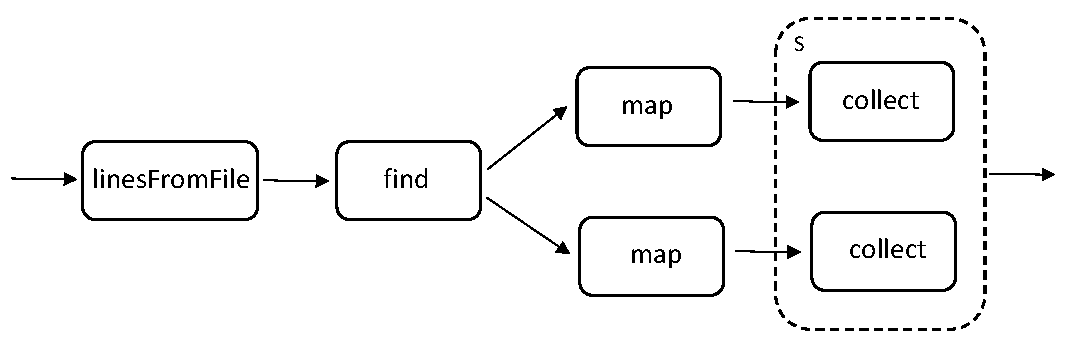
\includegraphics[width=\textwidth]{Figures/ExempleRuntimeExecution.pdf}
      \caption[Une repr\'esentation graphique d'un \TT{pipeline} compos\'e de quatre op\'erations.]{Une repr\'esentation graphique d'un \TT{pipeline} compos\'e de quatre op\'erations ex\'ecut\'ees en parall\`ele. Du parall\'elisme de flux est appliqu\'e sur les deux premi\`eres op\'erations et du parall\'elisme de donn\'ees est appliqu\'e sur les derni\`eres op\'erations. Le~\texttt{S}~sur la boite pointill\'ee \`a droite indique un \emph{Stage}.}
       \label{ExempleRuntimeExecution.fig}
\end{figure}


La figure~\ref{ExempleRuntimeExecution.fig} montre la repr\'esentation graphique d'un \TT{Pipeline} compos\'e des op\'erations d\'ecrites dans le listing~\ref{listingExampleImplementationPpFf}.
 

La classe \TT{Pipeline} de \TT{PpFf} repr\'esente l'entit\'e principale de l'application. \`A l'ex\'ecution, un \TT{Pipeline} correspond \`a une classe \TT{ff\_pipeline} de \TT{FastFlow}. Un \TT{Pipeline} est compos\'e de plusieurs nœuds de type \TT{ff\_node} ou \TT{ff\_farm}. 

Dans un \TT{Pipeline}, la premi\`ere op\'eration est toujours une op\'eration d'entr\'ee, laquelle est impl\'ement\'ee sous forme d'un \TT{ff\_node}. Dans notre exemple, \TT{source} renvoie un flux s\'equentiel de lignes \`a partir d'un fichier. De plus, l'op\'eration d'entr\'ee a aussi la t\^ache d'envoyer un signal \TT{EOS} (\emph{\texttt{E}nd \texttt{O}f \texttt{S}tream}) lorsque la g\'en\'eration du flux d'entr\'ee est termin\'ee~: \TT{EOS} indique aux nœuds \TT{ff\_node}s de \TT{FastFlow} de terminer leur ex\'ecution apr\`es la r\'eception de celui-ci.

La classe repr\'esentant chaque nœud dans un \TT{Pipeline} contient les informations concernant son r\^ole dans la chaine de traitement. Par exemple, l'op\'eration \TT{find} du listing~\ref{listingExampleImplementationPpFf} a pour r\^ole de s\'electionner dans le flux seulement les mots qui ne sont pas vides. Ce r\^ole est d\'efini par l'utilisateur \`a la cr\'eation du \TT{Pipeline}, en fournissant une fonction ou une expression lambda \`a \TT{find}.


Les divers op\'erations d'un \TT{Pipeline} sont toujours ex\'ecut\'ees en parall\`ele~: dans \TT{FastFlow}, chaque \TT{ff\_node} est associ\'e \`a un \emph{thread} ind\'ependant, donc le mod\`ele de parall\'elisme de flux est appliqu\'e par d\'efaut. 

En outre, lorsqu'un appel \`a la m\'ethode \TT{parallel} est ajout\'e dans la chaine du traitement d'un \TT{Pipeline}, les op\'erations subs\'equentes sont ex\'ecut\'ees en parall\`ele, et ce en utilisant du parall\'elisme de donn\'ees. Dans l'exemple du listing~\ref{listingExampleImplementationPpFf}, les deux premi\`eres op\'erations sont ex\'ecut\'ees en parall\`ele, avec du parall\'elisme de flux, alors que du parall\'elisme de flux et du parall\'elisme de donn\'ees sont aussi utilis\'es pour les op\'erations suivantes (apr\`es \TT{parallel}). 

Dans l'impl\'ementation de \TT{PpFf}, le parall\'elisme de donn\'ees est mis en œuvre avec la classe \TT{ff\_farm} de \TT{FastFlow}. La cr\'eation du flux de traitement en utilisant le mod\`ele de parall\'elisme de donn\'ees est simple. Lorsque la m\'ethode \TT{parallel()} est invoqu\'ee, une instance de la classe \TT{ff\_farm} est ajout\'ee dans le \TT{Pipeline}. Pour chaque \emph{worker} de \TT{ff\_farm}, un nouveau \TT{ff\_pipeline} est cr\'e\'e. Les op\'erations ajout\'ees dans la chaine du traitement  sont ajout\'ees comme nœuds dans les nouveaux \TT{ff\_pipeline} cr\'e\'es. Par exemple, les op\'erations \TT{map} et \TT{collect} du listing~\ref{listingExampleImplementationPpFf} sont ajout\'ees dans le \TT{pipeline} de chaque \TT{worker} de \TT{ff\_farm}. 


\begin{figure}
\centering
     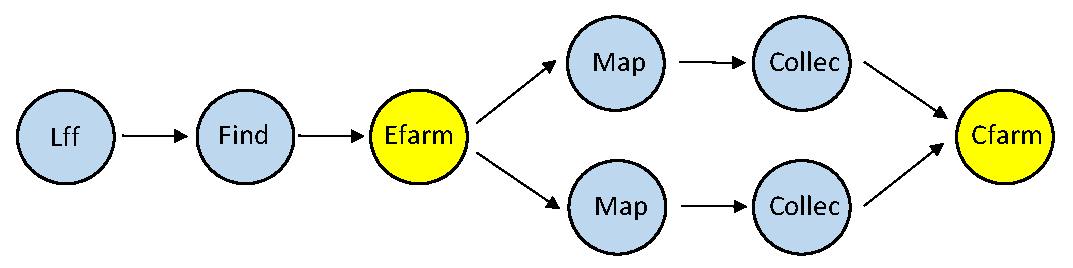
\includegraphics[width=\textwidth]{Figures/ExempleRuntimeExecutionFF.pdf}
      \caption[Une repr\'esentation graphique du listing~\ref{listingExampleImplementationPpFf} en \TT{FastFlow}.]{Une repr\'esentation graphique du listing~\ref{listingExampleImplementationPpFf} en \TT{FastFlow}. Les cercles bleus repr\'esentent les op\'erations sp\'ecifi\'ees par l'utilisateur : \TT{linesFromFile} (\texttt{Lff}), \TT{find} (\texttt{Find}), les deux \TT{map} (\texttt{Map}) et les deux \TT{collector} (\texttt{Collec}). Les cercles en jaunes repr\'esentent l'\emph{Emitter} et le \emph{Collector} du \TT{ff\_farm}.}
       \label{ExempleRuntimeExecutionFF.fig}
\end{figure}


La figure~\ref{ExempleRuntimeExecutionFF.fig} montre la repr\'esentation graphique du pipeline \TT{FastFlow} qui met en \oe{}uvre le pipeline \PpFf\ de la figure~\ref{ExempleRuntimeExecution.fig}. Chaque cercle est une classe de type \TT{ff\_node}. Les cercles en bleu repr\'esentent les op\'erations sp\'ecifi\'ees par l'utilisateur : \TT{linesFromFile} (Lff), \TT{find} (Find), les deux \TT{map} (Map) et les deux \TT{collector} (Collec). Les cercles en jaunes repr\'esentent l'\emph{Emitter} et le \emph{Collector} de l'objet \TT{ff\_farm}. 


L'ex\'ecution parall\`ele d'un flux est r\'ealis\'ee par l'ex\'ecution de la m\'ethode \TT{run\_and\_wait\_end()} de la classe \TT{ff\_pipeline} de \TT{FastFlow}. Chaque \TT{ff\_node} de \TT{ff\_pipeline} est une instance de la classe C++ \TT{ff\_node} qui ex\'ecute une boucle de traitement qui va comme suit:
\begin{itemize}
	\item obtient du canal d'entr\'ee (via un pointeur) un \'el\'ement \`a traiter;
	\item ex\'ecute le code sur l'\'el\'ement, code indiqu\'e dans la m\'ethode \TT{svc()};
	\item \'emet dans le canal de sortie (via un pointeur)  l'\'el\'ement produit.
\end{itemize}



Les nœuds d'un pipeline sont ex\'ecut\'es jusqu'\`a ce qu'ils re\c coivent le signal \TT{EOS}. \`A ce moment, tous les nœuds sont d\'etruits. Dans le cas de noeuds multiples associ\'es \`a du parall\'elisme de donn\'ees, le r\'esultat global de l'op\'eration est obtenu en combinant les r\'esultats des sous-flux produits par les divers fils d'ex\'ecution. Par exemple, chaque op\'eration \TT{collect} repr\'esent\'ee dans la figure~\ref{ExempleRuntimeExecution.fig} collecte le r\'esultat du traitement de chacun des sous-flux trait\'es dans un fil d'ex\'ecution ind\'ependant. Le r\'esultat global est obtenu via la classe \TT{Stage} qui combine ces r\'esultats interm\'ediaires, tel qu'expliqu\'e \`a la section~\ref{StagesDataParallel.sect}



